\documentclass[11pt, a4paper]{scrartcl}

% --packages--
\usepackage[utf8]{inputenc}
\usepackage[italian]{babel}
\usepackage{graphicx}
\usepackage{MnSymbol}
\setlength{\parindent}{0pt}
\def \a {\textsf{A}}

\title{\textbf{Smart House}}
\author{Mattia Curatitoli - 735722  Danilo Deponti - 737838} \date{}

\begin{document}
\maketitle
 
\section*{Introduzione}
L'invecchiamento della popolazione sta avendo un impatto sempre più significativo sul sistema sanitario. Per questo si cercano di trovare vie più efficienti per portare assistenza in casa alle persone bisognose.
Monitorare le attività umane ($ADL$) è diventato un aspetto fondamentale per costruire un ambiente intelligente atto a garantire il benessere degli anziani.
Uno degli approcci più promettenti ed economici è il monitoraggio delle attività tramite una rete wireless di sensori ($WSN$). In quanto molto flessibile e di facile sviluppo.
Sono stati sviluppati parecchi modelli che utilizzano sensori per monitorare le attività $ADL$, modelli come $Reti Bayesiane$ o $Conditional Random Fields$. In particolare, si è notato che $Hidden Markov Model$ ($HMM$) è un modello performante in questo dominio applicativo.
\section*{I sensori}
Sono stati utilizzati dataset presi da 2 appartamenti. Ogni appartamento contiene 2 dataset, il primo per le rilevazioni derivate dai sensori che monitorano le $ADL$, il secondo invece contiene le attività rilevate dai sensori.
Il dataset dei sensori è composto da righe corrispondenti all' intervallo di tempo nei quali i sensori sono stati attivi. Ogni riga contiene: $Start$ $time$, $End$ $time$, $Location$, $Type$, $Place$.
\begin{figure}[!ht]
\centering
 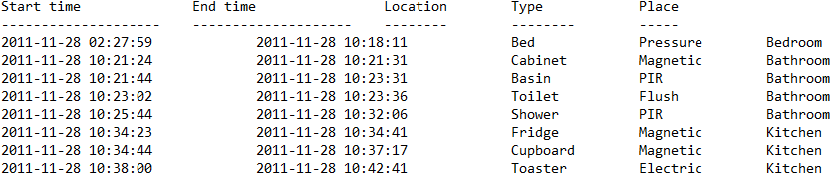
\includegraphics[scale=0.7]{Sensor.png} 
 \caption{Dataset iniziale dei sensori}
\label{fig:magn}
\end{figure}

Il dataset delle attività, invece, contiene l'intervallo di tempo ed il nome dell'attività rilevata.
Ogni attività è strettamente legata ai sensori. Ogni riga del dataset corrisponde ad un' attività ed ogni riga contiene: $Start$ $time$, $End$ $time$, $Activity$.

\begin{figure}[!ht]
\centering
 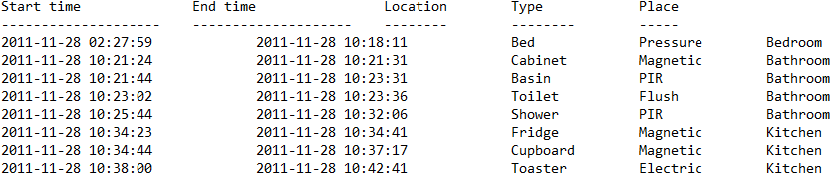
\includegraphics[scale=0.7]{Sensor.png} 
 \caption{Dataset iniziale delle attività}
\label{fig:magn}
\end{figure}


\section*{HMM}
Un $HMM$ ($Hidden$ $Markov$ $Model$) è un modello probabilistico definito da variabili osservabili $x_t$ e variabili nascoste $y_t$, dove $t$ indica il tempo. In questo caso le nostre variabili osservabili sono i sensori, mentre le vaariabili nascoste sono le attività. In un $HMM$ la variabile $y$ al tempo $t$, dipende solo dallo stato della variabile $y$ al tempo $t-1$. La variabile $x$ dipende solo dallo stato della variabile $y$ allo stesso istante $t$.


\begin{figure}[!ht]
\centering
 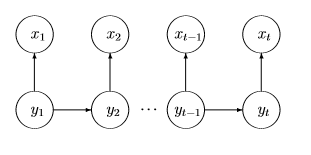
\includegraphics[scale=0.7]{HMM.png} 
 \caption{Hidden Markov Model}
\label{fig:magn}
\end{figure}

\section*{Il Software}

Il software è stato sviluppato in $Python$. Il software sviluppato permette di creare un $HMM$ partendo da una sequenza di rilevazioni prese da un appartamento. Si è deciso di trasformare le rilevazioni in formato $.txt$ in un formato più compatto ed ordinato, il $csv$. Come verrà spiegato dettagliatamente nel paragrafo successivo, il software analizza il file e calcola le probabilità iniziali, di transizione degli stati e di emissione degli eventi in base alle occorrenze all'interno del file. Successivamente, il software si avvarrà di una libreria chiamata $GHMM$, una libreria atta a creare modelli $HMM$, fare del $training$ su di essi e permette inoltre di inferire sl modello creato.
Su ogni file sono stati svolti controlli di consistenza sui dati rilevati( se il timestamp di inizio rilevazione è inferiore alla fine, se gli eventi sono temporalmente consecutivi ecc...).
Per la lettura del file dei sensori la tripla ($Location$, $type$, $place$) è stata utilizzata come chiave univoca per la definizione delle emissioni, verranno quindi considerati stati distinti per ogni nuova tripla rilevata all'interno del file.

\section*{Le funzioni}
Di seguito sono descritte le funzioni principali del software. In modo da illustrare dettagliatamente il metodo usato per creare le probabilità utilizzate per la creazione del modello.

\subsection*{obtainpadls}
La funzione $obtainpadls$ permette di ricavare le probabilità iniziali di ogni singola attività. Questa funzione conta semplicemente quante volte la stessa attività compare all'interno del file ed incrementa un contatore ad ogni rilevazione.

\subsection*{obtaintadls}
Questa funzione, invece, permette di ricavare la matrice delle transizioni per le $ADL$. $obtaintadls$ controlla, date tutte le volte che un attività accade in tempo $t_n$, quante volte ogni singola attività compare al tempo $t_(n+1)$. In modo da avere una matrice $nXn$ con la somma, per ogni attività, delle volte che le altre attività sono accadute successivamente.

\subsection*{normalizematrix e normalizelist}
Queste funzioni prendono semplicemente in  input le matrici e le liste create in precedenza e le normalizzano. In modo che la lista delle probabilità iniziali ed ogni riga della matrice delle transizioni abbiano come somma $1$. In questo modo otteniamo le matrici in funzione delle probabilità.

\subsection*{obtainosensadls}






\end{document}
